\documentclass[a4paper, 10pt]{article}
\setlength{\topmargin}{0in}
\setlength{\textheight}{8in}
\setlength{\oddsidemargin}{.1in}
\setlength{\textwidth}{6in}

\usepackage{multirow}
\usepackage{float}
\usepackage{array}
\usepackage[document]{ragged2e}
\usepackage{comment} 
\usepackage{subcaption}
\usepackage{amssymb,amsmath}
\usepackage[font={small,it}]{caption}

\usepackage{datetime}
\usepackage{tgbonum}

\newdateformat{mydate}{\monthname[\THEMONTH] \THEYEAR}

\newcolumntype{L}{>{\centering\arraybackslash}m{3cm}}

\newcommand{\tab}[1]{\hspace{.2\textwidth}\rlap{#1}}
\usepackage{graphicx}
\graphicspath{{images/}}

\begin{document}


\LARGE\title{Predicting Flight Delays With Increased Accuracy.}

\LARGE\author{\textbf{Esha Massand}\\
\date{\mydate\today}
\\\
}

\normalsize


\maketitle


\section*{Abstract}
\begin{justify}
The aim of the current project was to develop a model which could predict with high accuracy whether a flight departure would be delayed. The model is 99.3\% predictive to within 5 minute intervals (rather than 15 minute intervals). The proposed purpose of the work would be to reduce costs associated with delays and increase customer satisfaction by providing more accurate information about flight schedules. 
\end{justify}


\clearpage
\tableofcontents
\clearpage

\section{Variable Definitions}\label{variables}

\begin{tabular}{l p{11cm}  }
Year& Year\\
Quarter& Quarter (1-4)\\
Month& Month\\
DayofMonth& Day of Month\\
DayOfWeek& Day of Week\\
Carrier& Code assigned by IATA and commonly used to identify a carrier. As the same code may have been assigned to different carriers over time, the code is not always unique. For analysis, use the Unique Carrier Code\\
FlightNum& Flight Number\\
Origin& Origin Airport\\
Dest& Destination Airport\\
DepTime& Actual Departure Time (local time: hhmm)\\
DepDelay& Difference in minutes between scheduled and actual departure time. Early departures show negative numbers\\
DepDelay\_5min\_intervals & Departure Delay Indicator in 5 minute intervals. Early departures are also represented in this categorical variable\\
DepDel15& Departure Delay Indicator, 15 Minutes or More (1=Yes)\\
Distance& Distance between airports (miles)\\
State & State\\
Latitude & Latitude of State\\
Longitude & Longitude of State\\
\end{tabular}

\clearpage

\section{Introduction}\label{intro}

Approximately 22.5\% of flights were delayed in 2014 according to the U.S. Department of Transport (DOT). Large costs are associated with flight delays.  Delay also results in large inconveniences to customers and potential loss of their custom. The dataset at hand considers delay in 15 minute increments; a delay is recorded in the dataset only if the flight incurs a delay of greater than 15 minutes. When using these data in predictive modeling, I argue that this is not an accurate enough time-resolution. This approach does not consider the cascading effects of a shorter flight delay on subsequent connections, or the scheduled `tarmac time' for a flight upon arrival at it's destination. Since this is a real concerns for airlines and customers, the current report develops a model to predict flight delays with greater accuracy building on the current data that are available. 

\subsection{Exploration}
I began by exploring the United States Department of Transportation (DOT) dataset (found here: http://www.rita.dot.gov/bts/press\_releases/dot075\_15). The dataset itself contains information on the variables listed in section~\ref{variables} of this report (amongst others), from 1987 to 2015 across the USA. Variables with a high percentage missing data were not included in the analysis.

\vspace{5mm}
To better understand the dataset and which features may be useful for the predictive model, I used the Data Statistics Toolbox library in MATLAB to plot the data in question. To limit the scope of the project, the month of June 2015 was considered as a subset of the larger dataset. 

\begin{figure}[H]
\begin{center}
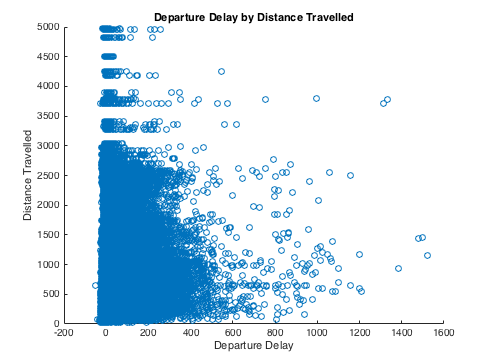
\includegraphics[scale=0.5]{departureDelayByDistanceTravelled}
\caption{Departure Delay by Distance.}
\label{departureDelayByDistanceTravelled}
\end{center}
\end{figure}

As can be seen from the scatter plot, there is a large variance in the departure delay times, the variance appears to be greater for flights under 3000 miles than over 3000 miles \footnote{To determine whether these data points were true outliers, a larger analysis over multiple years and months should be carried out. It would otherwise be difficult to determine whether or not these high variances were meaningful (and important for the model to account for), or spurious.}. 

\begin{figure}[H]
\begin{center}
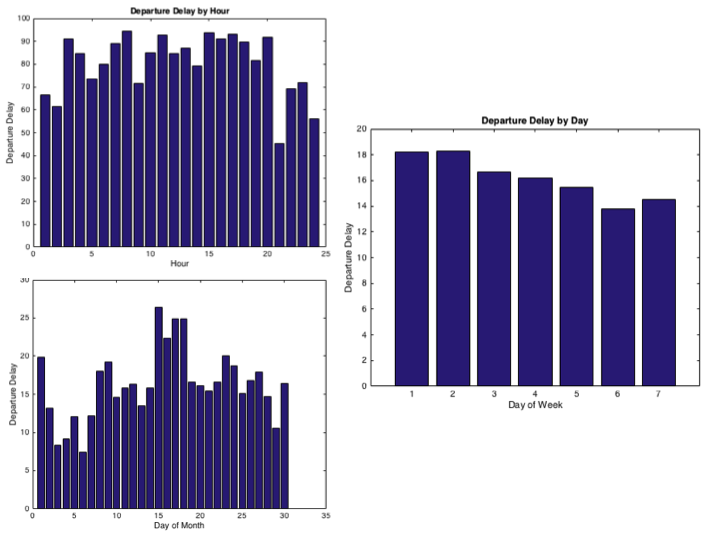
\includegraphics[scale=0.5]{explore}
\caption{Departure Delay by Hour, Day of Week and, Day of Month in June.}
\label{explore}
\end{center}
\end{figure}

We see that flights are less delayed after 8 pm and before 2 am. There is a clear pattern of increasing delay in flight departures between 5 am and 9 am, presumably because of the build up of depatures during the peak hours of the day. There is also a peak in departure delay between 3 pm and 8pm which is also in line with peak hours of the day.

\vspace{5mm}
Departure delays are most prominent early in the week (days 1 and 2), and tend to decrease on the 3-6th day of the week. The last day of the weekend on day 7, there is an increase in flight departure delays. This is what we could expect given peak travel during the weekend.

\vspace{5mm}
Departure delays are greatest mid month in June. There is also an interesting oscilating pattern in departure delays every 7 or so days. This is what we would expect given the weekend peak in travel. This is also in line with public holiday and vacation periods during June.

\begin{figure}[H]
\begin{center}
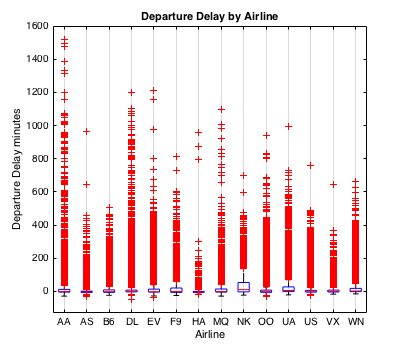
\includegraphics[scale=0.5]{departureDelayByAirline}
\caption{Departure Delay by Airline Carrier.}
\label{departureDelayByAirline}
\end{center}
\end{figure}

As was be expected, some airline carriers perform better in terms of departure delay performance than others.

\clearpage
To enrich the model with more data, I also explored the supplementary `airports.csv' file which included data on longitude and latitude of airports in the dataset. For the purposes of the current project, I focused on a smaller dataset from June 2015, and data from 2 airline carriers, \textbf{Alaska Airlines Inc}, and \textbf{Jet Blue Airways}. Together these departure delay data and airport coordinate data are presented below.

\begin{figure}[H]
\begin{subfigure}{.6\textwidth}
  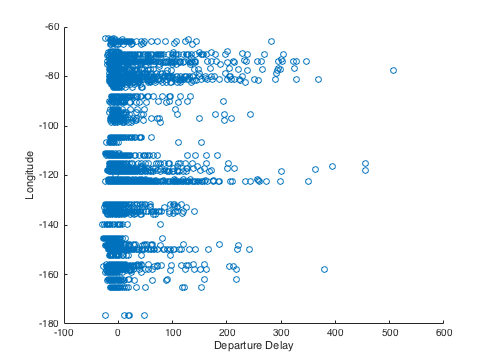
\includegraphics[width=.8\linewidth]{long2}
  \caption{Longitude Data and Delays in Departure Time.}
\end{subfigure}%
\begin{subfigure}{.6\textwidth}
  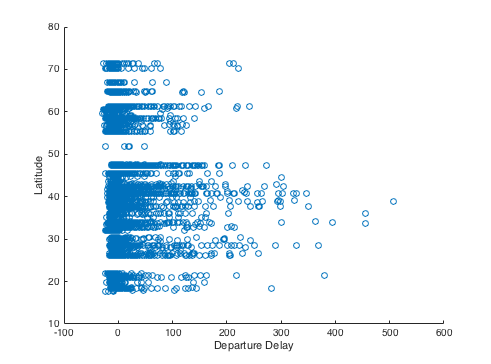
\includegraphics[width=.8\linewidth]{lat2}
  \caption{Latitude Data and Delays in Departure Time.}
\end{subfigure}
\end{figure}

As can be seen, there is a lot of variation in departure delays from the west coast (-180 longitude) to the east coast (-60 longitude) of the united states, with greater departure delays from central US, and east US. It is possible that this is because the east (New York, JFK for example) and regions in central US are `hubs' for travellers, attracting a greater volume of customers. There is also a wide variation in delays from the north (70) to southern parts (20) of the United States, with most delays originating from regions closer to the equator, presumably due to higher traffic compared to regions of greater latitude.

\subsection{Hypothesis}\label{hypothesis}
The aim of the current project was to develop a model which could predict with high accuracy whether a flight departure would be delayed to within 5 minute intervals, rather than the current 15 minute intervals. The proposed purpose of the work would be to reduce costs associated with delays and increase customer satisfaction by providing more accurate information about flight schedules. \\
The hypotheses for each variable were as follows:\\

\begin{tabular}{l p{11cm}  }
Day of month & The pattern should oscillate from low to high delays every 5-7 days to reflect weekend versus weekday. For certain months of the year, this may show a clearer pattern.\\
Day of week & Weekends are busier than weekdays\\
Hour of day & Flights during peak hours are busier than off peak hours\\
Carrier & Some carriers perform better than others\\
Flight Number & Certain flight numbers may be prone to delays due to inefficient scheduling by airlines\\
Origin & Some origin airports may perform better than others at getting flights to take off\\
Destination & Some destination airports may perform better than others with communicaton, having cascading effects on departure delays at the departure airport. \\
Departure Time & Some times of the day are busier than others\\
Distance & Flights that are further away have shorter delays\\
Latitude & Flights departing from areas closer to the equator have greater traffic volunes compared to regions much further north and consequently, will have greater delays\\
Longitude & Flights departing at an airport `hub' will have greater delays
\end{tabular}



\section{Method}
After exploration of the data on the U.S. DOT website data, I extracted variables of particular interest to build a predictive model of flight departure delays. The procedure to implement the model including loading in the June 2015 dataset, filtering out flights that were not carried by \textbf{Alaska Airlines Inc} or \textbf{Jet Blue Airways}, deleting outliers for departure delays, and projecting only variables that were useful predictors, or responses in the analysis. The feature selection process is explained next.

\subsection{Feature Selection}
The possible features from U.S. DOT are:
\begin{itemize}
\item{Day of Month}
\item{Day of Week}
\item{Carrier}
\item{Flight Number}
\item{Origin}
\item{Destination}
\item{Departure Time}
\item{Departure Delay in Minutes}
\item{Distance between Origin and Destination}
\end{itemize}

The features that were extracted from the airports.csv file, and combined to the dataset gathered from the U.S. DOT website were:
\begin{itemize}
\item{State}
\item{Latitude}
\item{Longitude}
\end{itemize}

\vspace{5mm}
These features formed the predictors for the model. Missing data for these features was $<$0.005\%. Any data rows with missing data were excluded from training and testing the model. 

\subsection{Preprocessing the Data}
In a preprocessing step, I computed a new variable to calculate a departure delay in 5 minute intervals, with early departures also being represented in a categorical variable called `DepDelay\_5min\_intervals'. This was the response feature for the model. There were 7 unique levels to the categorical variable and these were:
\begin{itemize}
\item{departed\_early\_greaterThan\_15}
\item{departed\_early\_10}
\item{departed\_early\_5}
\item{onTime}
\item{departed\_late\_5}
\item{departed\_late\_10}
\item{departed\_late\_greaterThan\_15}
\end{itemize}

\vspace{5mm}
Departure Delay variances were large, and to eliminate outliers from the model, delays that were $>$600 minutes were removed (in total this summed to 4 data points).

\subsection{Selecting a Model to Train}

\begin{figure}[H]
\begin{center}
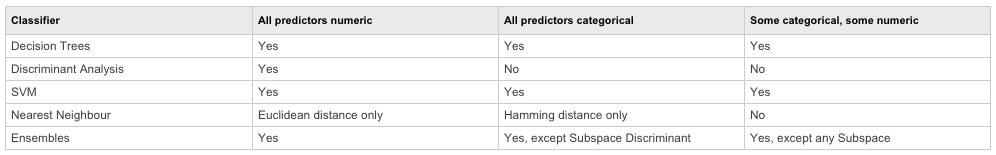
\includegraphics[scale=0.45]{classifiertypes}
\caption{Decision trees can handle a mixture of categorical and numerical data to build a model.}
\label{classifiertypes}
\end{center}
\end{figure}

\begin{figure}[H]
\begin{center}
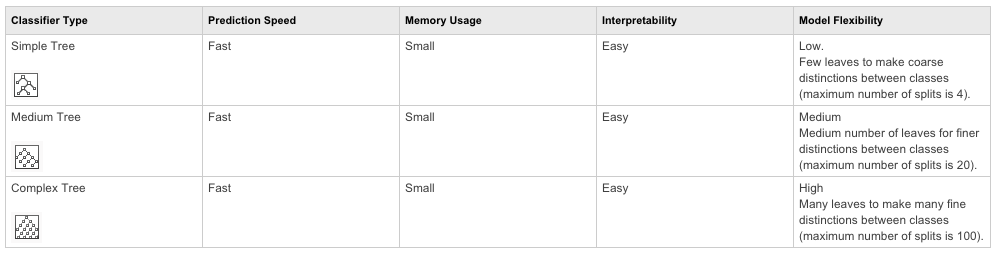
\includegraphics[scale=0.45]{decisiontrees}
\caption{Decision trees are fast, and complex trees have a high model flexibility.}
\label{decisiontrees}
\end{center}
\end{figure}

A decision tree was selected as an appropriate model for the dataset because this type of model can handle a mixture of categorical and numerical data, and complex trees have a high model flexibility.

\subsection{Model Training}
There were 11548 observations in the dataset with 13 predictors (listed above). The response variable was `departure delay in 5 minute intervals', which had 7 response classes. The MATLAB code for training the model can be seen in my GitHub repository here: https://github.com/BBK-SDP-2015-emassa01/Report-for-Spotify under the \texttt{longlat data} folder and in the \texttt{trainClassifierComplex.m} file).

\subsection{Model Performance: Iterations}

\begin{figure}[H]
\begin{center}
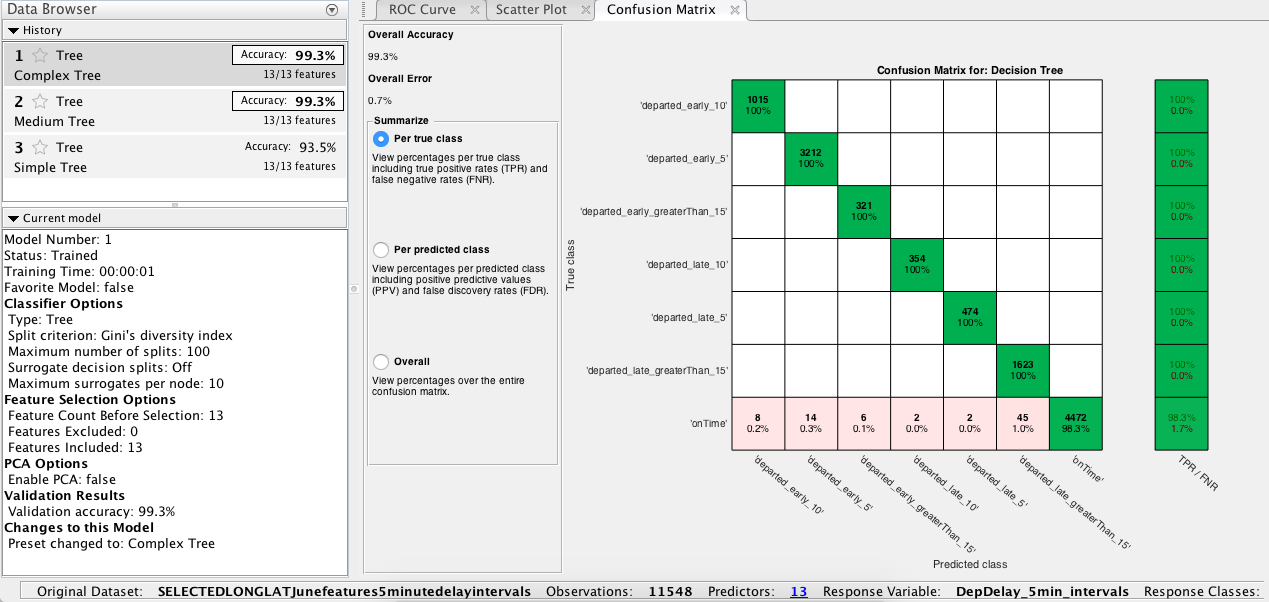
\includegraphics[scale=0.3]{3models}
\caption{Three iterations of the model were run; simple, medium and complex.}
\label{3models}
\end{center}
\end{figure}


I used the classificationLearner MATLAB application to run the models. The model that yielded greatest accuracy were the medium and complex decision trees, both yielding 99.3\% accuracy using 13 features listed above. Several other iterations of the model were run, but for brevity only these three are reported (for the remaining iterations and my workings for the current report please see: https://github.com/BBK-SDP-2015-emassa01/Report-for-Spotify).

\vspace{5mm}
The confusion matrix shows that the model works very well for 6 out of the 7 categories. The model has difficulty with flights that left `onTime', i.e., within 5 minutes of scheduled departure. The model tends to class these flights as `early' or `greater than 15 minutes late', so further refinement of the model is necessary. Perhaps with a larger data set.

\subsection{Validation Criteria}
Five-fold cross validation was used to prevent overfitting the model to the data, and to give an honest assessment of the true accuracy of the system. The purpose of cross validation is to ensure a diverse and more representative validation set to test the model. 

\vspace{5mm}
The code for the final Trained Classifier for the complex decision tree can be downloaded as a MATLAB workspace here: https://github.com/BBK-SDP-2015-emassa01/Report-for-Spotify/blob/master/longlat\%20data/trainedClassifierComplex.mat 



\subsection{Observations}

\begin{figure}[H]
\begin{center}
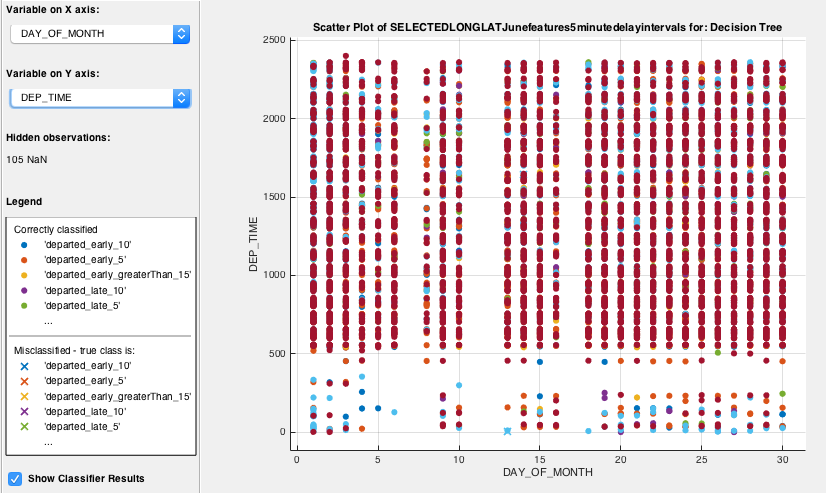
\includegraphics[scale=0.45]{4am}
\caption{Reduction in number of flights departing prior to 5 am.}
\label{4am}
\end{center}
\end{figure}
Whilst exploring the data, it became apparent that there are a reduced number of flights departing airports prior to 5 am. It is possible that this is due to scheduled staff shift-changes during these hours. These hours are not representative of the entire day's data. The data from this period of the day however, feed into the model generated and so may dilute the predictive power of the model. If I were to generate future models, I would focus on data gathered from around the same time of the day across multiple days to generate better models with greater predictive power.

\section{Conclusion}
When working through the dataset, there were several variables that I thought would assist with my research questions.  For example, gathering information about the size of the airport, and whether passengers were likely to be making a connection or not. Even small delays are, of course, more of a concern when having to make a connection. 

\vspace{5mm}
Weather information, or information pertaining to the cause of the delay was in most cases missing (90.14\%). However, weather information is a factor that would significantly impact trends in data gathered between summer and winter months. 

\end{document} 